\documentclass[a4paper, 14pt]{extarticle}

% Поля
%--------------------------------------
\usepackage{geometry}
\geometry{a4paper,tmargin=2cm,bmargin=2cm,lmargin=3cm,rmargin=1cm}
%--------------------------------------


%Russian-specific packages
%--------------------------------------
\usepackage[T2A]{fontenc}
\usepackage[utf8]{inputenc}
\usepackage[english, main=russian]{babel}
%--------------------------------------

\usepackage{textcomp}

% Красная строка
%--------------------------------------
\usepackage{indentfirst}
%--------------------------------------


%Graphics
%--------------------------------------
\usepackage{graphicx}
\graphicspath{ {./images/} }
\usepackage{wrapfig}
%--------------------------------------

% Полуторный интервал
%--------------------------------------
\linespread{1.3}
%--------------------------------------

%Выравнивание и переносы
%--------------------------------------
% Избавляемся от переполнений
\sloppy
% Запрещаем разрыв страницы после первой строки абзаца
\clubpenalty=10000
% Запрещаем разрыв страницы после последней строки абзаца
\widowpenalty=10000
%--------------------------------------

%Списки
\usepackage{enumitem}

%Подписи
\usepackage{caption}

%Гиперссылки
\usepackage{hyperref}

\hypersetup {
	unicode=true
}

%Рисунки
%--------------------------------------
\DeclareCaptionLabelSeparator*{emdash}{~--- }
\captionsetup[figure]{labelsep=emdash,font=onehalfspacing,position=bottom}
%--------------------------------------

\usepackage{tempora}

%Листинги
%--------------------------------------
\usepackage{listings}
\lstset{
  basicstyle=\ttfamily\footnotesize,
  %basicstyle=\footnotesize\AnkaCoder,        % the size of the fonts that are used for the code
  breakatwhitespace=false,         % sets if automatic breaks shoulbd only happen at whitespace
  breaklines=true,                 % sets automatic line breaking
  captionpos=t,                    % sets the caption-position to bottom
  inputencoding=utf8,
  frame=single,                    % adds a frame around the code
  keepspaces=true,                 % keeps spaces in text, useful for keeping indentation of code (possibly needs columns=flexible)
  keywordstyle=\bf,       % keyword style
  numbers=left,                    % where to put the line-numbers; possible values are (none, left, right)
  numbersep=5pt,                   % how far the line-numbers are from the code
  xleftmargin=25pt,
  xrightmargin=25pt,
  showspaces=false,                % show spaces everywhere adding particular underscores; it overrides 'showstringspaces'
  showstringspaces=false,          % underline spaces within strings only
  showtabs=false,                  % show tabs within strings adding particular underscores
  stepnumber=1,                    % the step between two line-numbers. If it's 1, each line will be numbered
  tabsize=2,                       % sets default tabsize to 8 spaces
  title=\lstname                   % show the filename of files included with \lstinputlisting; also try caption instead of title
}
%--------------------------------------

%%% Математические пакеты %%%
%--------------------------------------
\usepackage{amsthm,amsfonts,amsmath,amssymb,amscd}  % Математические дополнения от AMS
\usepackage{mathtools}                              % Добавляет окружение multlined
\usepackage[perpage]{footmisc}
%--------------------------------------

%--------------------------------------
%			НАЧАЛО ДОКУМЕНТА
%--------------------------------------

\begin{document}

%--------------------------------------
%			ТИТУЛЬНЫЙ ЛИСТ
%--------------------------------------
\begin{titlepage}
\thispagestyle{empty}
\newpage


%Шапка титульного листа
%--------------------------------------
\vspace*{-60pt}
\hspace{-65pt}
\begin{minipage}{0.3\textwidth}
\hspace*{-20pt}\centering

\includegraphics[width=\textwidth]{emblem}
\end{minipage}
\begin{minipage}{0.67\textwidth}\small \textbf{
\vspace*{-0.7ex}
\hspace*{-6pt}\centerline{Министерство науки и высшего образования Российской Федерации}
\vspace*{-0.7ex}
\centerline{Федеральное государственное автономное образовательное учреждение }
\vspace*{-0.7ex}
\centerline{высшего образования}
\vspace*{-0.7ex}
\centerline{<<Московский государственный технический университет}
\vspace*{-0.7ex}
\centerline{имени Н.Э. Баумана}
\vspace*{-0.7ex}
\centerline{(национальный исследовательский университет)>>}
\vspace*{-0.7ex}
\centerline{(МГТУ им. Н.Э. Баумана)}}
\end{minipage}
%--------------------------------------

%Полосы
%--------------------------------------
\vspace{-25pt}
\hspace{-35pt}\rule{\textwidth}{2.3pt}

\vspace*{-20.3pt}
\hspace{-35pt}\rule{\textwidth}{0.4pt}
%--------------------------------------

\vspace{1.5ex}
\hspace{-35pt} \noindent \small ФАКУЛЬТЕТ\hspace{80pt} <<Информатика и системы управления>>

\vspace*{-16pt}
\hspace{47pt}\rule{0.83\textwidth}{0.4pt}

\vspace{0.5ex}
\hspace{-35pt} \noindent \small КАФЕДРА\hspace{50pt} <<Теоретическая информатика и компьютерные технологии>>

\vspace*{-16pt}
\hspace{30pt}\rule{0.866\textwidth}{0.4pt}

\vspace{11em}

\begin{center}
\Large {\bf Лабораторная работа № 2} \\
\large {\bf по курсу <<Численные методы линейной алгебры>>} \\
\large <<Метод Гаусса и его модификации. Оценка погрешностей>>
\end{center}\normalsize

\vspace{8em}


\begin{flushright}
  {Студент группы ИУ9-72Б Старовойтов А. И. \hspace*{15pt}\\
  \vspace{2ex}
  Преподаватель Посевин Д. П.\hspace*{15pt}}
\end{flushright}

\bigskip

\vfill


\begin{center}
\textsl{Москва 2025}
\end{center}
\end{titlepage}
%--------------------------------------
%		КОНЕЦ ТИТУЛЬНОГО ЛИСТА
%--------------------------------------

\renewcommand{\ttdefault}{pcr}

\setlength{\tabcolsep}{3pt}
\newpage
\setcounter{page}{2}

\section{Задание}\label{Sect::task}

Реализовать четыре варианта метода Гаусса с перестановками и научиться оценивать
погрешность решения системы линейных уравнений для матриц произвольной
размерности.

\section{Реализация}\label{Sect::impl}

Исходный код программы представлен в листингах~\ref{lst:code1}--~\ref{lst:code7}.

\begin{figure}[!htb]
\begin{lstlisting}[language={},caption={Метод Гаусса},label={lst:code1}]
using Test
using Random
using LinearAlgebra

Random.seed!(42)

generate_matrix(n) = begin
    return rand(n, n)
end

@test generate_matrix(2) == [0.6293451231426089 0.47740714343281776; 0.4503389405961936 0.7031298490032014]

set_first_non_zero(i, A, b, perm) = begin
    A_copy = copy(A)
    b_copy = copy(b)
    n = size(A_copy, 1)

    if A_copy[i, i] != 0
        return A_copy, b_copy, perm
    end

    for j in (i+1):n
        if A_copy[j, i] != 0
            A_copy[i, :], A_copy[j, :] = A_copy[j, :], A_copy[i, :]
            b_copy[i], b_copy[j] = b_copy[j], b_copy[i]
            break
        end
    end

    return A_copy, b_copy, perm
end

@test set_first_non_zero(1, [0.0 1.0 1.0; 1.0 0.0 0.0; 0.0 2.0 2.0], [1.0, 2.0, 3.0], []) == ([1.0 0.0 0.0; 0.0 1.0 1.0; 0.0 2.0 2.0], [2.0, 1.0, 3.0], [])
@test set_first_non_zero(1, [2.0 1.0 1.0; 1.0 0.0 0.0; 0.0 2.0 2.0], [1.0, 2.0, 3.0], []) == ([2.0 1.0 1.0; 1.0 0.0 0.0; 0.0 2.0 2.0], [1.0, 2.0, 3.0], [])
@test set_first_non_zero(2, [1.0 1.0 1.0; 0.0 0.0 1.0; 0.0 3.0 2.0], [1.0, 2.0, 3.0], []) == ([1.0 1.0 1.0; 0.0 3.0 2.0; 0.0 0.0 1.0], [1.0, 3.0, 2.0], [])

exclude_ith_variable(i, A, b) = begin
    A_copy = copy(A)
    b_copy = copy(b)
    n = size(A_copy, 1)
    for j in (i+1):n
        l_ij = -A_copy[j, i] / A_copy[i, i]
        A_copy[j, :] += A_copy[i, :] * l_ij
        b_copy[j] += l_ij * b_copy[i]
    end
    return A_copy, b_copy
end

@test exclude_ith_variable(1, [1.0 1.0 1.0; 2.0 -1.0 1.0; 3.0 2.0 -1.0], [6.0, 3.0, 4.0]) == ([1.0 1.0 1.0; 0.0 -3.0 -1.0; 0.0 -1.0 -4.0], [6.0, -9.0, -14.0])
\end{lstlisting}
\end{figure}

% \newpage

\begin{figure}[!htb]
\begin{lstlisting}[language={},caption={Метод Гаусса (продолжение)},label={lst:code2}]
@test exclude_ith_variable(2, [1.0 1.0 1.0; 0.0 -3.0 -1.0; 0.0 -1.0 -4.0], [6.0, -9.0, -14.0]) == ([1.0 1.0 1.0; 0.0 -3.0 -1.0; 0.0 0.0 -3.6666666666666665], [6.0, -9.0, -11.0])
forward_pass(A, b, diagonal_element_choosing_strategy) = begin
    perm = collect(1:size(A, 1))
    start_max_element = maximum(A)
    current_max_element = start_max_element
    for i in 1:size(A, 1)
        A, b, perm = diagonal_element_choosing_strategy(i, A, b, perm)
        A, b = exclude_ith_variable(i, A, b)
        current_max_element = max(current_max_element, maximum(A))
    end
    growth_factor = current_max_element / start_max_element
    solution_error_estimate = growth_factor * eps(Float64) * size(A, 1) * cond(A, 2)
    return A, b, perm, solution_error_estimate
end

@test forward_pass([1.0 1.0 1.0; 2.0 -1.0 1.0; 3.0 2.0 -1.0], [6.0, 3.0, 4.0], set_first_non_zero) == ([1.0 1.0 1.0; 0.0 -3.0 -1.0; 0.0 0.0 -3.6666666666666665], [6.0, -9.0, -11.0], [1, 2, 3], 3.009212689604127e-15)

backward_pass(A, b) = begin
    n = size(A, 1)
    x = zeros(n)
    for i in n:-1:1
        x[i] = (b[i] - sum(A[i, j] * x[j] for j in (i+1):n; init=0.0)) / A[i, i]
    end
    return x
end

@test backward_pass([1.0 1.0 1.0; 0.0 -3.0 -1.0; 0.0 0.0 -3.6666666666666665], [6.0, -9.0, -11.0]) == [1.0, 2.0, 3.0]

restore_order(x, perm) = begin
    result = similar(x)
    for i in eachindex(x)
        result[perm[i]] = x[i]
    end
    return result
end

@test restore_order([6.0, -9.0, -11.0], [3, 2, 1]) == [-11.0, -9.0, 6.0]

gauss(A, b, diagonal_element_choosing_strategy) = begin
    A, b, perm, solution_error_estimate = forward_pass(A, b, diagonal_element_choosing_strategy)
    x = backward_pass(A, b)
    x = restore_order(x, perm)
    return x, solution_error_estimate
end

@test gauss([1.0 1.0 1.0; 2.0 -1.0 1.0; 3.0 2.0 -1.0], [6.0, 3.0, 4.0], set_first_non_zero) == ([1.0, 2.0, 3.0], 3.009212689604127e-15)

\end{lstlisting}
\end{figure}

\begin{figure}[!htb]
\begin{lstlisting}[language={},caption={Метод Гаусса (продолжение)},label={lst:code3}]
set_max_element_in_column(i, A, b, perm) = begin
    A_copy = copy(A)
    b_copy = copy(b)

    _, max_element_index = findmax(abs(A_copy[j, i]) for j in i:size(A_copy, 1))
    max_element_index += i - 1

    A_copy[i, :], A_copy[max_element_index, :] = A_copy[max_element_index, :], A_copy[i, :]
    b_copy[i], b_copy[max_element_index] = b_copy[max_element_index], b_copy[i]
    return A_copy, b_copy, perm
end

@test set_max_element_in_column(1, [1.0 1.0 1.0; 2.0 -1.0 1.0; 3.0 2.0 -1.0], [6.0, 3.0, 4.0], []) == ([3.0 2.0 -1.0; 2.0 -1.0 1.0; 1.0 1.0 1.0], [4.0, 3.0, 6.0], [])
@test set_max_element_in_column(2, [1.0 1.0 1.0; 2.0 -1.0 1.0; 3.0 2.0 -1.0], [6.0, 3.0, 4.0], []) == ([1.0 1.0 1.0; 3.0 2.0 -1.0; 2.0 -1.0 1.0], [6.0, 4.0, 3.0], [])

@test gauss([1.0 1.0 1.0; 2.0 -1.0 1.0; 3.0 2.0 -1.0], [6.0, 3.0, 4.0], set_max_element_in_column) == ([1.0, 2.0, 3.0], 2.4564265188457937e-15)

swap_columns(A, i, j) = begin
    A_copy = copy(A)
    A_copy[:, [i, j]] = A_copy[:, [j, i]]
    return A_copy
end

@test swap_columns([1.0 1.0 1.0; 2.0 -1.0 1.0; 3.0 2.0 -1.0], 1, 2) == [1.0 1.0 1.0; -1.0 2.0 1.0; 2.0 3.0 -1.0]

set_max_element_in_row(i, A, b, perm) = begin
    A_copy = copy(A)
    b_copy = copy(b)
    perm_copy = copy(perm)
    _, max_element_index = findmax(abs(A_copy[i, j]) for j in i:size(A_copy, 2))
    max_element_index += i - 1

    A_copy = swap_columns(A_copy, i, max_element_index)
    perm_copy[i], perm_copy[max_element_index] = perm_copy[max_element_index], perm_copy[i]

    return A_copy, b_copy, perm_copy
end

@test set_max_element_in_row(1, [1.0 2.0 3.0; 4.0 5.0 6.0; 7.0 8.0 9.0], [1.0, 2.0, 3.0], [1, 2, 3]) == ([3.0 2.0 1.0; 6.0 5.0 4.0; 9.0 8.0 7.0], [1.0, 2.0, 3.0], [3, 2, 1])

@test gauss([1.0 1.0 1.0; 2.0 -1.0 1.0; 3.0 2.0 -1.0], [6.0, 3.0, 4.0], set_max_element_in_row) == ([1.0, 2.0, 3.0], 3.009212689604127e-15)

set_max_element_overall(i, A, b, perm) = begin
\end{lstlisting}
\end{figure}

\begin{figure}[!htb]
\begin{lstlisting}[language={},caption={Метод Гаусса (продолжение)},label={lst:code5}]
    A_copy = copy(A)
    b_copy = copy(b)
    perm_copy = copy(perm)
    max_element = 0.0
    max_element_coords = (0, 0)
    for row in i:size(A_copy, 1)
        for col in i:size(A_copy, 2)
            if abs(A_copy[row, col]) > max_element
                max_element = abs(A_copy[row, col])
                max_element_coords = (row, col)
            end
        end
    end
    max_i, max_j = max_element_coords
    A_copy = swap_columns(A_copy, i, max_j)
    perm_copy[i], perm_copy[max_j] = perm_copy[max_j], perm_copy[i]
    A_copy[i, :], A_copy[max_i, :] = A_copy[max_i, :], A_copy[i, :]
    b_copy[i], b_copy[max_i] = b_copy[max_i], b_copy[i]
    return A_copy, b_copy, perm_copy
end

@test gauss([1.0 1.0 1.0; 2.0 -1.0 1.0; 3.0 2.0 -1.0], [6.0, 3.0, 4.0], set_max_element_overall) == ([1.0, 2.0, 3.0], 2.4564265188457937e-15)

get_diagonal_dominance_degree(A) = begin
    n = size(A, 1)
    min_degree = Inf
    for i in 1:n
        diagonal_element = abs(A[i, i])
        off_diagonal_sum = sum(abs(A[i, j]) for j in 1:n if j != i)
        degree = diagonal_element - off_diagonal_sum
        min_degree = min(min_degree, degree)
    end
    return min_degree
end

@test get_diagonal_dominance_degree([7.0 2.0 1.0; 1.0 -8.0 2.0; 0.0 1.0 6.0]) == 4.0

build_matrix_with_dominance(n, dominance) = begin
    A = zeros(n, n)
    S = max(n - 1.0, -dominance + 1.0)
    c = S / (n - 1.0)
    for i in 1:n
        for j in 1:n
            if j != i
                A[i, j] = c
            end
        end
        A[i, i] = S + dominance
    end
    for i in 2:n
        A[i, i] += rand(1:100)
\end{lstlisting}
\end{figure}

\begin{figure}[!htb]
\begin{lstlisting}[language={},caption={Метод Гаусса (продолжение)},label={lst:code6}]
    end

    return A
end

@test get_diagonal_dominance_degree(build_matrix_with_dominance(3, 4.0)) == 4.0
@test get_diagonal_dominance_degree(build_matrix_with_dominance(3, -80.0)) == -80.0

struct TestResult
    error_classic::Float64
    error_row::Float64
    error_column::Float64
    error_both::Float64
    error_library::Float64
    diagonal_dominance::Float64
    estimate_classic::Float64
    estimate_row::Float64
    estimate_column::Float64
    estimate_both::Float64
end

results = TestResult[]

euqlid_norm(x, y) = sqrt(sum((x - y).^2))

for i in 1:100
    want_dominance = rand(-100:100)
    A = build_matrix_with_dominance(5, want_dominance)
    # A = generate_matrix(5)
    x = rand(5)
    b = A * x

    classic, estimate_classic = gauss(A, b, set_first_non_zero)
    row, estimate_row = gauss(A, b, set_max_element_in_row)
    column, estimate_column = gauss(A, b, set_max_element_in_column)
    both, estimate_both = gauss(A, b, set_max_element_overall)
    library = A \ b
    error_classic = euqlid_norm(x, classic)
    error_row = euqlid_norm(x, row)
    error_column = euqlid_norm(x, column)
    error_both = euqlid_norm(x, both)
    error_library = euqlid_norm(x, library)
    # println([error_classic, error_row, error_column, error_both, error_library])

    diagonal_dominance = get_diagonal_dominance_degree(A)

    push!(results, TestResult(error_classic, error_row, error_column, error_both, error_library, diagonal_dominance, estimate_classic, estimate_row, estimate_column, estimate_both))
end

for res in results
    println(res)
\end{lstlisting}
\end{figure}

\begin{figure}[!htb]
\begin{lstlisting}[language={},caption={Метод Гаусса (продолжение)},label={lst:code7}]
end

using PyCall
pygui(:tk)
using PyPlot

dominances = [r.diagonal_dominance for r in results]
errors_classic = [r.error_classic for r in results]
errors_row = [r.error_row for r in results]
errors_column = [r.error_column for r in results]
errors_both = [r.error_both for r in results]
errors_library = [r.error_library for r in results]
estimates_classic = [r.estimate_classic for r in results]
estimates_row = [r.estimate_row for r in results]
estimates_column = [r.estimate_column for r in results]
estimates_both = [r.estimate_both for r in results]

figure(figsize=(12, 8))

subplot(1, 2, 1)
scatter(dominances, errors_classic, alpha=0.6, label="Classic", s=20)
scatter(dominances, errors_row, alpha=0.6, label="Row pivot", s=20)
scatter(dominances, errors_column, alpha=0.6, label="Column pivot", s=20)
scatter(dominances, errors_both, alpha=0.6, label="Both pivot", s=20)
scatter(dominances, errors_library, alpha=0.6, label="Library", s=20)
xlabel("Diagonal Dominance")
ylabel("Error (Euclidean norm)")
title("Error vs Diagonal Dominance")
legend()
grid(true, alpha=0.3)
yscale("log")

subplot(1, 2, 2)
scatter(dominances, estimates_classic, alpha=0.6, label="Classic", s=20)
scatter(dominances, estimates_row, alpha=0.6, label="Row pivot", s=20)
scatter(dominances, estimates_column, alpha=0.6, label="Column pivot", s=20)
scatter(dominances, estimates_both, alpha=0.6, label="Both pivot", s=20)
xlabel("Diagonal Dominance")
ylabel("Error estimate")
title("Error estimate vs Diagonal Dominance")
legend()
grid(true, alpha=0.3)
yscale("log")

savefig("gauss_methods_comparison.png", dpi=150)
show()

\end{lstlisting}
\end{figure}

\clearpage
\section{Результаты}\label{Sect::res}

Результат запуска представлен на рисунке~\ref{fig:img4}.

\begin{figure}[!htb]
	\centering
	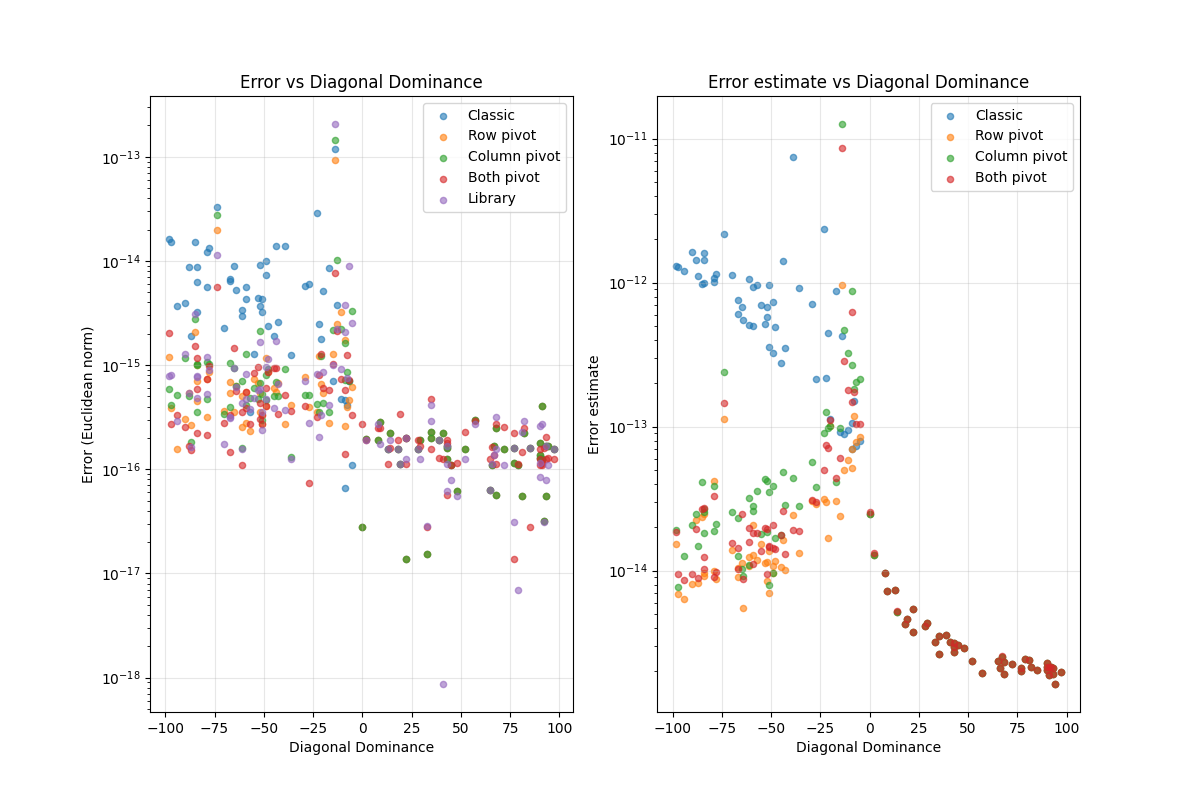
\includegraphics[width=0.8\textwidth]{img4}
\caption{Результат}
\label{fig:img4}
\end{figure}

\clearpage
\section{Выводы}\label{Sect::fin}

В результе выполнения данной лабораторной работы были реализованы классический
метод Гаусса, метод Гаусса с перестановками по столбцам, по строкам, по столбцам
и строкам одновременно для действительных квадратных матриц произвольной
размерности n. Построены графики зависимости абсолютной погрешности от степени
диагонального преобладания матрицы.

\end{document}
